\documentclass[12pt, a4paper]{article}
\usepackage{graphicx}
\usepackage{amsmath}
\usepackage[colorlinks=true, urlcolor=blue, linkcolor=red]{hyperref}
\usepackage{float}
\usepackage[utf8]{inputenc}
\usepackage[english]{babel}
\usepackage[top=2cm, bottom=2cm, left=2cm, right=2cm]{geometry}
\usepackage{booktabs}
\usepackage{biblatex}
\usepackage{csquotes}
\usepackage{tabularx, booktabs, tikz}
\usetikzlibrary{shapes.misc} % For rounded rectangles
% \bibliographystyle{ieeetr}
\addbibresource{refs.bib}

\title{Probing Graphene's Anomalous Quantum Hall Effect via Relativistic Electron Beam Scattering}
\author{Nathan Daniel Alspaugh, Juan Pablo Sojo, Mateo Peñaranda, \\Valeria Quintero, Juliana Taboada, Laura Díaz, \\Nairon Barrios, Samuel Correa, Isabella Altamar}
\date{\today}

\begin{document}

\maketitle

% Introduction
\section{Introduction}
The Quantum Hall Effect (QHE) is a phenomenon where the electrical conductivity of a material becomes quantized into discrete steps under strong magnetic fields. Usually, materials have to be supercooled to be able to observe these effects but it has been discovered that graphene can produce these same effects at room temperature \cite{Novoselov2007}. Unlike conventional materials, graphene's electrons behave as massless \textit{Dirac fermions}, leading to a "half-integer" QHE where conductivity plateaus occur at values of \(\sigma_{xy} = \pm(4e^2/h)(n + 1/2)\) instead of integers \cite{hsu2010anomalous}. This anomaly arises from graphene's hexagonal and plain atomic structure, where electrons follow the relativistic Dirac equation \cite{semenoff1984condensed}.

% Why We to Go to DESY
\section{Why We Want to Go to DESY}
DESY represents the chance to step into a world we've only dreamed of, a place where real science happens, where light unravels the mysteries of the universe. Coming from a country where advanced research infrastructure like particle accelerators isn't yet a reality, this opportunity means more than just pursuing a project. It's about experiencing cutting-edge science firsthand, and bringing that knowledge back to inspire and educate our community, students, teachers, and young minds who've never seen this kind of possibility up close. For us, DESY could be the start of something far greater, the beginning of our journey as scientists and changemakers.

\section{Hypothesis}
Directing DESY's electron/positron beam into a graphene sheet, will result in a pattern formed by the dispersion of Dirac fermions that can be measured through energy changes in the exiting beam, allowing for further understanding of graphene's properties and the Quantum Hall Effect.




% Methodology
\section{Experiment and Methodology}
The main objective of this experiment is to observe and test if the Quantum Hall Effect can be reproduced in graphite through an electron/positron beam. We believe that when the beam passes through the graphene sample, the electrons will scatter off the graphene's Dirac fermions, producing a unique scattering pattern that can be analyzed to extract information about the QHE. This experiment will also provide insights into the fundamental physics of graphene.

\subsection{Landau Levels in Graphene}
Landau levels (LLs) are quantized energy states that electrons occupy when subjected to a perpendicular magnetic field \cite{landau1930diamagnetismus}. In conventional materials, these levels arise from the cyclotron motion of electrons, where their classical circular orbits become quantized due to quantum mechanics. However, graphene's unique electronic structure, governed by the relativistic Dirac equation for massless fermions, leads to fundamentally distinct LLs behavior.
\begin{figure}[ht!]
    \centering
    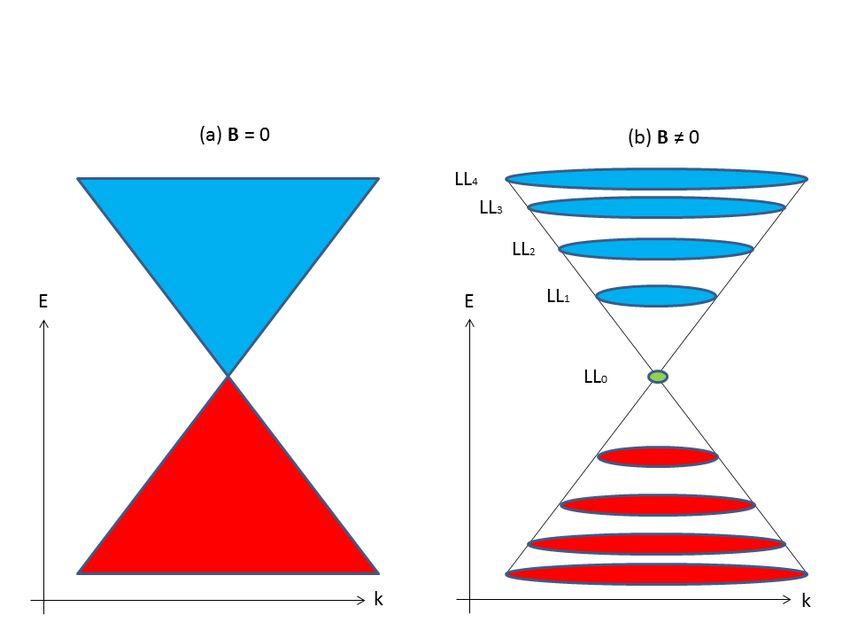
\includegraphics[width=0.8\textwidth]{images/levels.png}
    \caption{Graphene's Landau levels and their quantization under a magnetic field. \cite{li2007observation}}
    \label{fig:levels}
\end{figure}
When a magnetic field \(B\) is applied perpendicular to graphene's plane, the Lorentz force confines the Dirac fermions (graphenes' electrons) into discrete orbits. Solving the Dirac equation under these conditions yields the following energy spectrum:
\begin{equation}
    E_n = \text{sgn}(n)\hbar v_F \sqrt{2eB|n|}, \quad n = 0, \pm1, \pm2, \ldots
\end{equation}

The \(\sqrt{B|n|}\) dependence is a hallmark of graphene's relativistic nature. In non-relativistic materials (e.g., semiconductors), LLs scale linearly with \(B\) and \(n\): \(E_n \propto B(n + 1/2)\). Graphene's square-root relationship arises because its electrons obey the Dirac equation, which inherently links energy to the square root of momentum. This leads to unequally spaced LLs (e.g., \(E_1 - E_0 \neq E_2 - E_1\)) and the anomalous half-integer Quantum Hall Effect. The \(\text{sgn}(n)\) term ensures symmetry between electron (\(n > 0\)) and hole (\(n < 0\)) states, a direct consequence of graphene's bipartite lattice structure and Dirac cone geometry.

\begin{figure}[ht!]
    \centering
    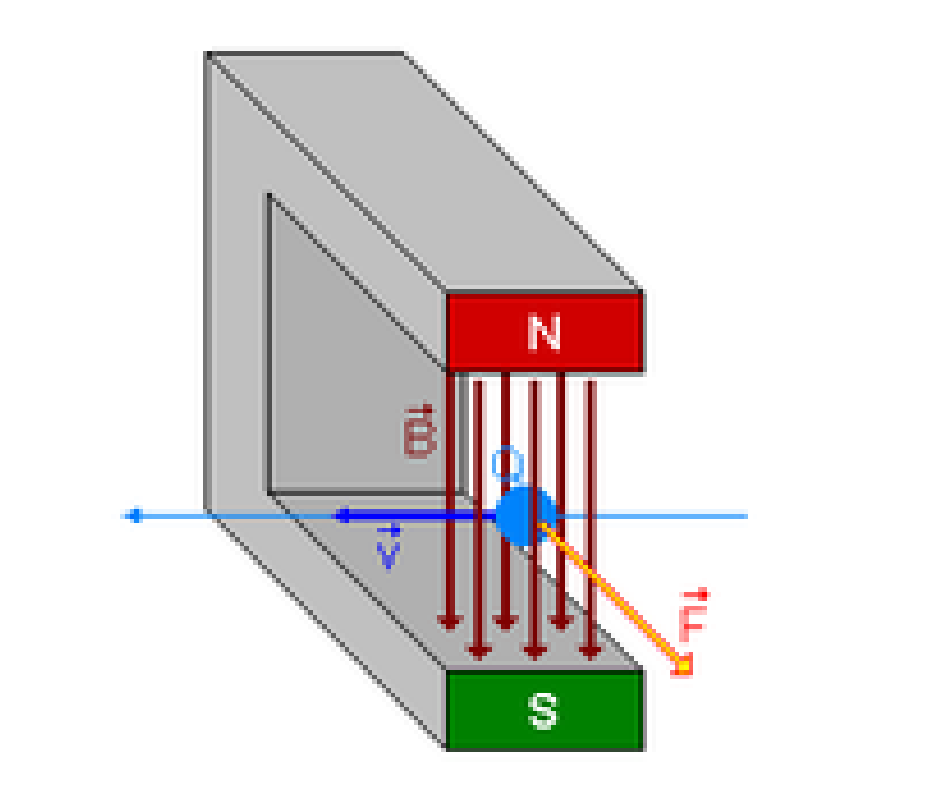
\includegraphics[width=0.4\textwidth]{images/lorenz.png}
    \caption{Lorenz force acting on electrons in a magnetic field, leading to quantized Landau levels in graphene.}
    \label{fig:lorenz}
\end{figure}
\subsection{Hall Conductivity Quantization}
The transverse (Hall) conductivity \(\sigma_{xy}\) becomes quantized in integer multiples of \(e^2/h\), a fundamental consequence of topology and gauge invariance \cite{france2025electrically}. The Quantum Hall Effect (QHE) in graphene exhibits a hallmark deviation from conventional materials: its Hall conductivity \(\sigma_{xy}\) quantizes at \textit{half-integer} multiples of \(4e^2/h\), expressed as:
\begin{equation}
    \sigma_{xy} = \pm \frac{4e^2}{h} \left(n + \frac{1}{2}\right), \quad n = 0, \pm1, \pm2, \ldots
\end{equation}
This anomalous quantization arises from two unique features of graphene:

\begin{itemize}
    \item \textbf{Fourfold Degeneracy (\(4e^2/h\)):} Each Landau level in graphene accommodates four independent electron states due to its two spin orientations (spin-up/spin-down) and two valleys (\(K\) and \(K'\) points in the Brillouin zone). This degeneracy multiplies the conventional conductance quantum \(e^2/h\) by 4.

    \item \textbf{Half-Integer Offset (\(n + 1/2\)):} The \(1/2\) shift originates from the Berry phase \(\pi\) acquired by Dirac fermions completing a cyclotron orbit. In graphene, the honeycomb lattice's symmetry imposes a geometric phase of \(\pi\) on circulating electrons, effectively altering the boundary conditions for quantization. This contrasts with non-relativistic materials, where the Berry phase is zero and conductivity quantizes at integers (\(n\)) \cite{M_V_Berry_1980}.
\end{itemize}

The filling factor \(\nu\), defined as \(\nu = n_e h / eB\) (where \(n_e\) is the electron density), determines the occupancy of Landau levels. In graphene, the relationship \(\nu = \pm4(n + 1/2)\) leads to conductivity plateaus at \(\nu = \pm2, \pm6, \pm10, \ldots\). These plateaus correspond to fully filled Landau levels, where scattering is suppressed, and \(\sigma_{xy}\) becomes \textit{universally precise}, independent of material defects or sample geometry.

\subsection{Experimental Design}
DESY's infrastructure is perfect for this study. The 1-6 GeV/c electron beam provides relativistic particles whose energies align with graphene's Dirac fermion dynamics. DESY's 1.35 T dipole electromagnet, enables the strong magnetic fields required to produce Landau quantization - the formation of discrete energy levels in graphene. With the use of silicone beam telescopes that allow the tracking of particle trajectories and lead-glass calorimeters to measure energy deposition, this setup allows us to correlate scattering patterns with graphene's LLs. The experiment directs DESY's electron beam through a suspended graphene sample (1 cm x 1 cm) under DESY's dipole magnet (Fig. \ref{fig:setup}). The magnetic field induces Landau levels in graphene, altering the beam's scattering profile. The key components include:

\begin{itemize}
    \item \textbf{Graphene Sample}: Monolayer (commercially sourced).
    \item \textbf{Collminator}: Filters beam, ensuring greater accuracy in scattering measurements.
    \item \textbf{Dipole Magnet}: Generates 1.35 T field perpendicular to the graphene plane.
    \item \textbf{Beam Telescopes}: Track scattering for later analysis.
    \item \textbf{Calorimeters}: Measure energy loss via lead-glass detectors.
\end{itemize}

\begin{figure}[ht!]
    \centering
    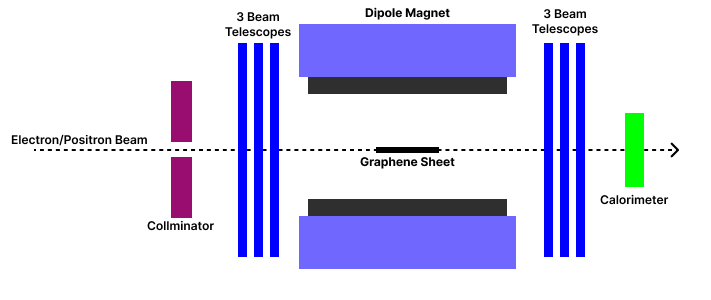
\includegraphics[width=0.8\textwidth]{images/experiment.png}
    \caption{DESY beamline with graphene sample, dipole magnet alignment, detection system.}
    \label{fig:setup}
\end{figure}
\subsection{Parameter Space}
The experiment varies three key parameters to map graphene's Quantum Hall response under relativistic beam conditions. These parameters were chosen to isolate the effects of Landau quantization, relativistic coupling, and particle-antiparticle symmetry:

\begin{table}[H]
    \centering
    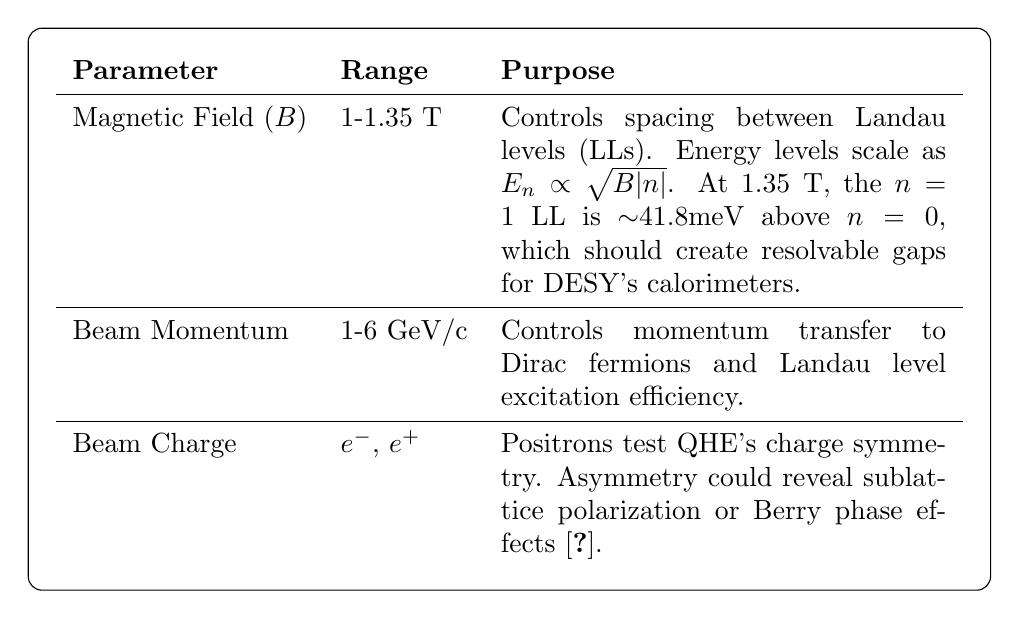
\begin{tikzpicture}
        \node [rectangle, rounded corners=5pt, draw, inner sep=10pt] { % Rounded border
            \begin{tabularx}{0.95\textwidth}{l l X} % Reduced width for border spacing
                \textbf{Parameter}     & \textbf{Range}   & \textbf{Purpose}                                                                                                                                                                                                           \\
                \midrule
                Magnetic Field (\(B\)) & 1-1.35 T         & Controls spacing between Landau levels (LLs). Energy levels scale as \(E_n \propto \sqrt{B|n|}\). At 1.35 T, the \(n=1\) LL is \(\sim\)41.8meV above \(n=0\), which should create resolvable gaps for DESY's calorimeters. \\
                \midrule
                Beam Momentum          & 1-6 GeV/c        & Controls momentum transfer to Dirac fermions and Landau level excitation efficiency.                                                                                                                                       \\
                \midrule
                Beam Charge            & \(e^-\), \(e^+\) & Positrons test QHE's charge symmetry. Asymmetry could reveal sublattice polarization or Berry phase effects \cite{LIU2017}.                                                                                                \\
            \end{tabularx}
        };
    \end{tikzpicture}
    \caption{Experimental parameters for graphene QHE investigation.}
    \label{tab:params}
\end{table}

By combining these parameters, we will recreate graphene's Quantum Hall plateaus (\(\sigma_{xy} = \pm2, \pm6, \ldots \times 4e^2/h\)) and test theoretical predictions under controlled conditions. For example, high \(B\) and low beam energy isolate \(n=0\) LL behavior, while positron beams explore antimatter analogs of Dirac fermion dynamics.

\section{Materials and Budget}
A detailed cost breakdown is available in our \href{https://docs.google.com/spreadsheets/d/1yHHGXo7aPC6-99GpaHHJ5hi_KQ2__5M-3WwTXWNNCyk/edit?usp=sharing}{Google Sheets}.

\section{Community Impact}
Over the past few years, we've visited several towns and places across the Caribbean region of Colombia, teaching children, especially older students, about math and physics in ways that feel interesting and exciting. Our goal has been to spark their curiosity and help them see that science and innovation isn't out of reach, that they too can pursue it. In a country where the shortage of engineers and scientists holds back development, we think and believe that inspiring the next generation is a step toward changing that. With every workshop, conversation, and experiment, we are building a stronger community, one where more young minds see a future in STEM fields.

% References
\printbibliography

\end{document}